\chapter{Estado del arte}\label{estado-del-arte}

En este capítulo se hace una breve revisión de los fundamentos del aprendizaje por refuerzo y del actual estado del arte, presentando un panorama general de los métodos y utilidades que se abordan en este trabajo.\\

Como se presentó en el punto \ref{motivacion} este trabajo presenta una solución que combina el aprendizaje por refuerzo con un vehículo dentro de un simulador para recorrer un circuito siguiendo una franja en el suelo. En este capítulo se recogen algunos de los métodos planteados así como las ventajas e inconvenientes de cada uno de ellos hasta el uso actual.\\

%%%%%%%%%%%%%%%%%%%%%%%%%%%%%%%%%%%%%%%%%%%%%%%%%%%%%%%%%%%%%%%%%%%%%%%%%%%%%%%%%%%%%%%%%%%%%%%%%%%%%%%%%%%%%%%%%%%%%%%%%%%%%%%%%%
\section{Aprendizaje por refuerzo}

Existen diferentes áreas de aprendizaje automático que permiten a un sistema generar una salida dada una entrada desconocida. En función del problema que se quiere solucionar, los entrenamientos en aprendizaje automático generan una u otra salida como puede ser un valor numérico, una probabilidad, una imagen (dentro del campo de la visión por computador), o una \textit{recompensa}. Es en este punto donde se encuentra la rama del \textit{aprendizaje por refuerzo} (\textit{reinforcement learning} o RL) que tiene un enfoque psicológico en el proceso de entrenamiento del algoritmo. En este aspecto se diferencia de los métodos de entrenamiento supervisados y es el propio agente el que se encarga de encontrar la mejor relación de parámetros para la solución del problema.\\

El aprendizaje por refuerzo puede definirse como: aprender qué hacer o cómo relacionar las situaciones (o \textit{estados}) con las \textit{acciones}, con el objetivo de maximizar una señal numérica de \textit{recompensa}. En este ámbito se describe uno de los elementos principales del aprendizaje, \textit{el agente}. El agente debe ser capaz de adquirir información del entorno y tomar decisiones que afecten a su estado. No se le dice qué acciones debe tomar, sino que debe descubrir qué acciones producen la \textit{mayor recompensa} cuando se llevan a cabo. Estas acciones pueden afectar no solo a la recompensa inmediata sino también a la siguiente situación y, a través de ella, a todas recompensas venideras.\\

Las tareas de toma de decisiones secuenciales cubren una amplia gama de posibles aplicaciones como: la robótica, asistencia sanitaria, las redes inteligentes, videojuegos, finanzas, conducción autónoma y muchas otras.\\

El aprendizaje por refuerzo proporciona a los agentes la capacidad de realizar experimentos para comprender mejor su entorno, lo que les permite aprender incluso relaciones causales de alto nivel. Las mejoras en \textit{renderizadores} visuales y motores de física permiten replicar cada vez con más fiabilidad entornos reales donde dejar que los agentes exploren y aprendan la mejor política o combinación de parámetros para aprender la tarea en cuestión. En la figura \ref{fig:dqn_hide-seek} se ilustra un entorno de pruebas del juego del 'pilla-pilla' donde los agentes que se esconden pueden mover paneles para ocultarse mejor. Pasados muchos episodios, los agentes rastreadores aprenden a mover esos paneles para encontrar a sus rivales.\\

\begin{figure}[!ht]
    \centering 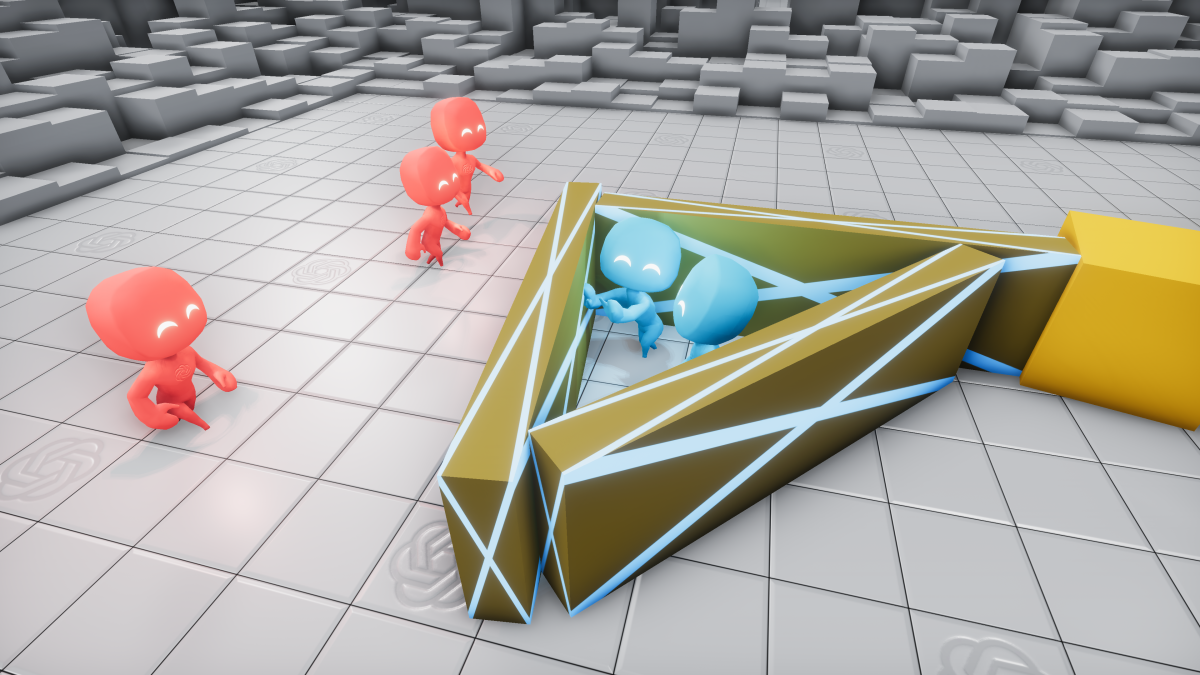
\includegraphics[width=0.6\columnwidth]{./figures/chapter_2/drl_hide_seek.png}
    \caption{Juego de "pilla-pilla". Unos agentes buscan y otros se esconden.}\label{fig:dqn_hide-seek}
\end{figure}

En el ámbito concreto que ocupa este Trabajo Fin de Máster, combinar este aprendizaje con un vehículo para solucionar el problema de control visual de completar una vuelta al circuito, supone un entorno de pruebas seguro donde el vehículo puede llegar a los límites admitidos y permite reiniciarse el entorno de simulación si llega a un extremo no deseado.\\

Aún quedan retos por delante para que esto sea posible en el mundo real, pero se está progresando en la idea de que los agentes aprendan los principios fundamentales del mundo a través de la observación y la acción. Esto permitirá aproximarse a sistemas de inteligencia artificial que aprendan y actúen de manera más humana en entornos cada vez más complejos.


%%%%%%%%%%%%%%%%%%%%%%%%%%%%%%%%%%%%%%%%%%%%%%%%%%%%%%%%%%%%%%%%%%%%%%%%%%%%%%%%%%%%%%%%%%%%%%%%%%%%%%%%%%%%%%%%%%%%%%%%%%%%%%%%%%
\subsection{Comportamiento recompensado} \label{comportamiento_recompensado}

\noindent
La esencia del aprendizaje por refuerzo es aprender a través de la interacción con el entorno, observando las consecuencias de haber realizado una acción para poder alterar su propio comportamiento en respuesta a las recompensas recibidas. Este paradigma hereda de la psicología y es conocido como \textit{ensayo-error} siendo una de las principales características en el campo del aprendizaje por refuerzo.\\

Como se explica en \cite{miles_brundage}, la interacción con el entorno es llevada a cabo por un \textit{agente}, controlado por algoritmos de aprendizaje automático que observa el estado $s_t$ de su entorno en un instante $t$. El agente interactúa con el entorno realizando una acción $a_t$ en el estado $s_t$. Cuando el agente ha realizado la acción $a_t$, el entorno y el agente transitan a un nuevo estado $s_{t+1}$ basado en el estado actual y la acción elegida. La mejor secuencia de acciones está determinada por las recompensas que ofrece el entorno.\\

El objetivo del agente es \textit{aprender una política} o estrategia que maximice la recompensa. El reto del aprendizaje por refuerzo es conseguir que el agente aprenda de las consecuencias de las acciones en el entorno a través de \textit{ensayo-error} ya que no existe un método de transición entre estados. Este bucle de \textit{percepción-acción-aprendizaje}, explicado en \cite{miles_brundage}, puede verse en la figura \ref{fig:percepcion-accion-aprendizaje}.

\begin{figure}[!ht]
    \centering 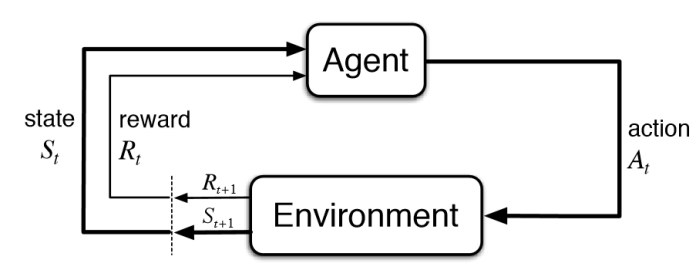
\includegraphics[width=0.6\columnwidth]{./figures/chapter_2/reinforcement-learning-diagram.jpg}
    \caption{Bucle de percepción-acción-aprendizaje llevado a cabo por el agente.\label{fig:percepcion-accion-aprendizaje}}
\end{figure}

\noindent
Estas dos características (la búsqueda a través de \textit{ensayo-error} y la recompensa) son las más diferenciales del aprendizaje de refuerzo.


%%%%%%%%%%%%%%%%%%%%%%%%%%%%%%%%%%%%%%%%%%%%%%%%%%%%%%%%%%%%%%%%%%%%%%%%%%%%%%%%%%%%%%%%%%%%%%%%%%%%%%%%%%%%%%%%%%%%%%%%%%%%%%%%%%
\subsection{Soluciones basadas en matrices o tablas}

Uno de los tipos de soluciones del aprendizaje por refuerzo es aquel en el que el estado y los espacios de acción son lo suficientemente pequeños para que las funciones de valor aproximado sean representadas como matrices o tablas. En estos casos, los métodos suelen encontrar soluciones o la función de valor óptima y la política óptima. Los tipos de soluciones basados en tablas se mencionan en \cite{sutton_barto} y  son los siguientes:\\

\begin{itemize}
    \item \textbf{\textit{Multi-armed bandits}}~\cite{multi_armed}: Denominado así por analogía con máquinas tragaperras (bandido con un solo brazo) con la salvedad de que se tienen \textit{k} palancas en lugar de una. La selección de una acción es como una tirada en una máquina siendo las mejores recompensas los mejores premios. El objetivo es concentrarse en las máquinas que retornan mejores premios (valores) descartando las que retornan peores.\\
    
    \item \textbf{Procesos de decisión finitos de Markov (MDP)}~\cite{markov_decision_process}: Este caso implica también una retroalimentación evaluativa (como el caso anterior) y además una asociativa. Es una formalización de la tomar de decisiones secuenciales donde la elección de distintas acciones en diferentes situaciones hacen que los resultados no solo influyan en las recompensas inmediatas sino que también en las futuras.\\

    \item \textbf{Programación Dinámica (DP)}~\cite{dynamic_programming}: Conjunto de algoritmos que pueden ser utilizados para calcular políticas óptimas requiriendo de un modelo muy preciso del entorno. Este método resuelve problemas MDP. Es un algoritmo que se toma como base para la comprensión del resto de algoritmos, siendo estos intentos por mejorar el coste computacional y la suposición del modelo perfecto del entorno que se impone en la programación dinámica.\\

    \item \textbf{Métodos de Monte Carlo}~\cite{multi_armed}: Este método se usa para resolver el MDP. No requiere conocimiento del entorno y logra comportamientos muy buenos. Se basa en el promedio de los resultados de las muestras. Conceptualmente es sencillo pero no es adecuado para el cálculo incremental paso a paso.\\

    \item \textbf{Aprendizaje de Diferencia Temporal}~\cite{temporal_difference_learning}: Es un método más novedoso. Siendo una combinación de la idea de Monte Carlo y programación dinámica puede aprender directamente de la experiencia en bruto sin un modelo de la dinámica del entorno. Igualmente, se usan para resolver problemas MDP. Son más complejos de analizar.\\
\end{itemize}

%%%%%%%%%%%%%%%%%%%%%%%%%%%%%%%%%%%%%%%%%%%%%%%%%%%%%%%%%%%%%%%%%%%%%%%%%%%%%%%%%%%%%%%%%%%%%%%%%%%%%%%%%%%%%%%%%%%%%%%%%%%%%%%%%%
\subsection{Métodos de solución aproximada}

En muchas de las tareas en la que se pretende aplicar aprendizaje por refuerzo, el espacio de estados es combinatorio y enorme: ingentes cantidades de imágenes tomadas de distintas cámaras. En tales casos, no puede esperarse encontrar una política óptima o una función de valor óptima incluso con un límite de tiempo infinito. En contraste con el método anterior el objetivo es encontrar una buena \textit{solución aproximada} utilizando recursos computacionales limitados.\\

Para tomar decisiones sensatas en grandes conjuntos de estados es necesaria la generalización. ¿Cómo puede la experiencia con un subconjunto limitado de estados producir una buena aproximación sobre un subconjunto mucho más grande?. Tal y como se menciona en \cite{sutton_barto}, utilizando \textit{funciones de aproximación}.\\

Existen diversos tipos de funciones de aproximación como:\\
\begin{itemize}
    \item \textbf{Predicción de valores}: usado en general en cualquier tipo de aprendizaje supervisado como árboles de decisión, regresión multivariante, etc, donde suele emplearse la métrica de la raíz del error cuadrático medio (RMSE) para la evaluación de las medidas.\\
    \item \textbf{Métodos de descenso-de gradiente}: Está entre los métodos más comunes de aproximación y es una de las piezas claves del aprendizaje profundo. Se calcula el error a través de las derivadas parciales en sentido opuesto al flujo de la red neuronal.\\
    \item \textbf{Métodos lineales}: Es un caso particular del método del descenso del gradiente donde la función de aproximación es una función lineal.
\end{itemize}

%%%%%%%%%%%%%%%%%%%%%%%%%%%%%%%%%%%%%%%%%%%%%%%%%%%%%%%%%%%%%%%%%%%%%%%%%%%%%%%%%%%%%%%%%%%%%%%%%%%%%%%%%%%%%%%%%%%%%%%%%%%%%%%%%%
\section{Algoritmos clásicos de aprendizaje por refuerzo} \label{algoritmos_clasicos_de_apredizaje_por_refuerzo}

En el aprendizaje por refuerzo el objetivo es aprender sin tener un modelado completo del entorno. Sin embargo, las interacciones con el entorno pueden ser usadas para aprender funciones de valor, políticas y, también, modelos.\\

En general existen dos aproximaciones para solventar problemas de aprendizaje por refuerzo:\\

\begin{itemize}
    \item Métodos que \textbf{no} están basados en modelos.
    \item Métodos basados en modelos.
\end{itemize}

%%%%%%%%%%%%%%%%%%%%%%%%%%%%%%%%%%%%%%%%%%%%%%%%%%%%%%%%%%%%%%%%%%%%%%%%%%%%%%%%%%%%%%%%%%%%%%%%%%%%%%%%%%%%%%%%%%%%%%%%%%%%%%%%%%
\subsection{Métodos sin modelos}

\noindent
Los métodos que no están basados en modelos aprenden directamente de las interacciones con el entorno, como pueden ser: los métodos basados en \textit{funciones de valor} (\textit{value functions}), la \textit{búsqueda de políticas} (\textit{policy search}) o métodos híbridos como el \textit{actor-crítico} (\textit{actor-critic}).\\

\begin{itemize}
\item \textbf{Funciones de valor}: Estos métodos están basados en la estimación del valor (rendimiento esperado) de estar en un estado $s$ dado. Se denomina función de \textit{valor-estado} $V^{\pi}(s)$. La política óptima se define como $\pi^*$. La función $Q^{\pi}(s,a)$ representa la función de calidad o \textit{state-action-value} (similar a $V^{\pi}$). La mejor política dará como resultado la mejor $Q^{\pi}(s,a)$. Esta función de calidad se mejora por diversos métodos de estimación dando lugar a la función denominada $Q-learning$\cite{christopher_watkins} y al algoritmo SARSA\cite{miles_brundage} (\textit{state-action-reward-state-action}) que sigue la ecuación:

    $$
    Q^{\pi}(s_t,a_t) \leftarrow Q^{\pi}(s_t,a_t) + \alpha \delta.
    $$
    
    \noindent
    Donde:
    \begin{itemize}
        \item $\alpha \rightarrow$ es la tasa de aprendizaje,
        \item $\delta \rightarrow$ es el error en la diferencia temporal (TD).
    \end{itemize}
    
     El valor $Q-learning$ se aproxima directamente a $Q^*$ y se encuentra a base de iteraciones con una evaluación  y mejora de las políticas que mejora la estimación de la \textit{función de valor}. A medida que la estimación mejora la política puede mejorarse eligiendo acciones basadas en la \textit{función de valor} actualizada.\\

    \item \textbf{Métodos de búsqueda de políticas}: No necesitan mantener un modelo de la \textit{función de valor} sino que se busca directamente una política óptima $\pi^*$. Las redes neuronales que codifican las políticas han tenido excelentes resultados usando en el entrenamiento ambos métodos: sin el uso del gradiente\cite{faustino_gomez} y basado en gradiente\cite{jan_peters}. El primero de ellos cubre eficazmente los parámetros cuando las dimensiones son reducidas pero con superficies grandes, el entrenamiento basado en gradiente es el mejor método actualmente para la mayoría de los algoritmos de aprendizaje por refuerzo profundo (\textit{Deep Reinforcement Learning}, (DRL)) cuando las políticas tienen un gran número de parámetros. Los métodos que no están basados en gradientes requieren búsquedas heurísticas para encontrar la mejor política pero, tienen como ventaja que también puede optimizar políticas no diferenciables.\\
    
    Las \textit{políticas de gradientes} \cite{satinder_singh} proporcionan una tasa de aprendizaje muy fuerte para mejorar políticas que llevan asociadas parámetros. La configuración más común de aprendizaje por refuerzo sin modelos es el uso del algoritmo de \textit{Monte Carlo}.\\
    
    \item Los métodos híbridos de actor-crítico (\textit{actor-critic}): combinan los valores con una representación explícita de la política. El \textit{actor} (política) aprende utilizando la retroalimentación del crítico (valor). En este proceso, los métodos compensan la desviación de reducción de los gradientes con las políticas con introducción de sesgo a partir de las funciones de valor.
\end{itemize}


%%%%%%%%%%%%%%%%%%%%%%%%%%%%%%%%%%%%%%%%%%%%%%%%%%%%%%%%%%%%%%%%%%%%%%%%%%%%%%%%%%%%%%%%%%%%%%%%%%%%%%%%%%%%%%%%
\subsection{Métodos basados en modelos}\label{metodos_basados_en_modelos}

Pueden simular transiciones usando el modelo aprendido~\cite{pieter_abbeel} que se traduce en una mayor eficiencia en la muestra. Estos métodos basados en modelos son particularmente importantes en entornos donde cada interacción con el entorno es especialmente costosa aunque introduce más complejidad en la creación y estructura del sistema (es más delicado porque al existir más parámetros el modelo puede contener errores). La solución a los problemas basados en modelos que se aporta en esta nueva etapa es el uso de las redes neuronales profundas que permiten crear modelos muy complejos y ricos de manera eficiente y que se explican con más detalle a continuación.

%%%%%%%%%%%%%%%%%%%%%%%%%%%%%%%%%%%%%%%%%%%%%%%%%%%%%%%%%%%%%%%%%%%%%%%%%%%%%%%%%%%%%%%%%%%%%%%%%%%%%%%%%%%%%%%%
\section{Aprendizaje profundo en aprendizaje por refuerzo}  

Denominado como \textit{aprendizaje por refuerzo profundo} (\textit{Deep Reinforcement Learning}, DRL en adelante), muchos de los éxitos de esta técnica se han basado en la \textit{ampliación de los trabajos previos} de aprendizaje por refuerzo \textit{a problemas de alta dimensión} permitiendo el aprendizaje de representaciones de características de baja dimensión así como la aproximación funcional de las redes neuronales~\cite{kay_arulkumaran}. Mediante el aprendizaje de la representación se hace frente al problema de la maldición de la dimensionalidad~\cite{naveen_venkat} que ocurría en los métodos basados en tablas y los tradicionales no paramétricos. El uso de redes neuronales convolucionales (\textit{convolutional neural network}, CNN) hace que puedan utilizarse como componentes de los agentes permitiéndoles aprender directamente de las imágenes crudas (componentes visuales de alta dimensión) o con menor procesamiento. En general, el aprendizaje por refuerzo profundo trata de aproximar una política óptima de $\pi^*$ o las funciones de valor óptimo $V^*$, $Q^*$ y $A^*$.

\hfill\break
\noindent
Los trabajos actuales se basan mayoritariamente en métodos basados en gradiente~\cite{gradient} dado que proporcionan una fuerte señal de aprendizaje. El éxito del DRL radica en el aprendizaje de la representación y la aproximación a las funciones. Este auge en el aprendizaje profundo ha inspirado nuevas formas de pensar y trabajar sobre el aprendizaje profundo lo que lleva a revisar las funciones de valor y búsqueda de políticas. Una de las más conocidos es \textit{Deep Q-network} (DQN).

%%%%%%%%%%%%%%%%%%%%%%%%%%%%%%%%%%%%%%%%%%%%%%%%%%%%%%%%%%%%%%%%%%%%%%%%%%%%%%%%%%%%%%%%%%%%%%%%%%%%%%%%%%%%%%%%
\subsection{Métodos no basados en modelos}

Al igual que en la sección \ref{algoritmos_clasicos_de_apredizaje_por_refuerzo}, se visitan los métodos basados en valores y en políticas:\\

\begin{itemize}
    \item \textbf{Métodos basados en funciones de valor}: Desde los primeros métodos de función de valor en DRL, que tomaban estados simples como entrada, los métodos actuales son ahora capaces de abordar entornos visual y conceptualmente complejos.\\
    
    El algoritmo DQN se convirtió en uno de los más populares en esta evolución en el uso de redes neuronales ya que logró conseguir \textit{records} de puntuación en los procesos de aprendizaje llevados a cabo en la videoconsola Atari~\cite{volodymyr_mnih_koray_kavukcuoglu}, ~\cite{volodymyr_mnih_david_silver} comparables con un jugador profesional utilizando imágenes en escala de gris como entrada (figura \ref{fig:dqn}). Cada una de las capas convolucionales completamente conectadas procesan estas imágenes que codifican los efectos de las acciones en su salida.
    
    \begin{figure}[!ht]
        \centering 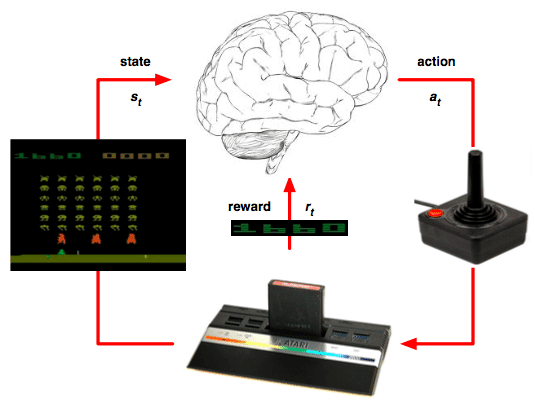
\includegraphics[width=0.6\columnwidth]{./figures/chapter_2/dqn_atari.png}
        \caption{
            \label{fig:dqn}
                Bucle de percepción-acción-aprendizaje llevado a cabo por el agente para la resolución de juegos en la videoconsola Atari.
        }
    \end{figure}
    
    \item \textbf{Métodos basados en políticas}: Los métodos de búsqueda de políticas tienen como objetivo encontrar directamente las políticas por medio de métodos o bien \textit{libres de gradientes} o \textit{basados en gradientes}. Antes del actual aumento de interés en DRL, varios métodos en este ámbito evitaron el algoritmo de retropropagación o propagación hacia atrás (en inglés, \textit{backpropagation}) comúnmente utilizado en favor de los algoritmos evolutivos que potencialmente pueden ser distribuidos a escalas mayores que las técnicas que se basan en gradientes.\\
    
    \item \textbf{Métodos del actor crítico (\textit{Actor-critic})}: Combina los beneficios de los métodos de búsqueda de políticas con lo aprendido en las funciones de valor y son capaces de aprender de los errores retornados de TD~\cite{eric_kolve}. En los últimos años, los métodos de DRL de actores críticos se han ampliado desde el aprendizaje de tareas de física simulada a tareas reales de navegación visual robótica, directamente desde los píxeles de la imagen. Un desarrollo más reciente de este tipo de métodos son los gradientes determinísticos (\textit{Deterministic Policy Gradients}, DPG en adelante) de las políticas que extiende los teoremas de política de gradientes. Una de las mayores ventajas es que, mientras que los gradientes de políticas estocásticas se integran tanto en los espacios de estados como en los de acción, los DPG solo se integran en los primeros requiriendo menos muestras en problemas con grandes espacios de acción.
\end{itemize}

%%%%%%%%%%%%%%%%%%%%%%%%%%%%%%%%%%%%%%%%%%%%%%%%%%%%%%%%%%%%%%%%%%%%%%%%%%%%%%%%%%%%%%%%%%%%%%%%%%%%%%%%%%%%%%%%
\section{Investigación actual y retos}

Existen múltiples áreas activas de investigación acerca de diferentes métodos y maneras de alcanzar un aprendizaje por refuerzo:\\

\begin{itemize}
    \item \textbf{Aprendizaje por refuerzo basado en modelo}: Mencionado en el punto \ref{metodos_basados_en_modelos}, permite aprender los modelos de transiciones que dispone el entorno pero sin la interacción directa con él~\cite{thomas_b_sch}. No asume conocimiento a priori. Sin embargo, puede incorporar información para acelerar el proceso de aprendizaje. Dado que es poco realista realizar millones de experimentos con un robot en un tiempo razonable existen varios enfoques para aprender modelos predictivos utilizando información de los píxeles. Se incorpora información de alta dimensión que se reduce con autocodificadores (\textit{autoencoders}). En esencia, si se puede aprender un modelo suficientemente preciso del entorno entonces los controladores más sencillos pueden ser usados para controlar un robot directamente desde las imágenes de la cámara. Utilizando aprendizaje profundo es más viable simular entornos sobre cientos y cientos de muestras que, la mayoría de las veces, son caras o difíciles de conseguir. Es una vía muy eficiente de entrenar modelos y mejorar la eficiencia de los parámetros. Un ejemplo de uso de este tipo del aprendizaje por refuerzo basado en modelo es el presentado por Łukasz Kaiser y su equipo~\cite{rl_basado_en_modelo} donde se pretende enseñar a un agente a completar videojuegos de la Atari a través de muy pocas visualizaciones para intentar igualar en tiempo de aprendizaje a un humano, en apenas 2 horas. El trabajo se llama SimPLe y en la figura \ref{fig:rl_simple} puede verse el bucle principal del programa.\\
    
    \begin{figure}[!ht]
        \centering 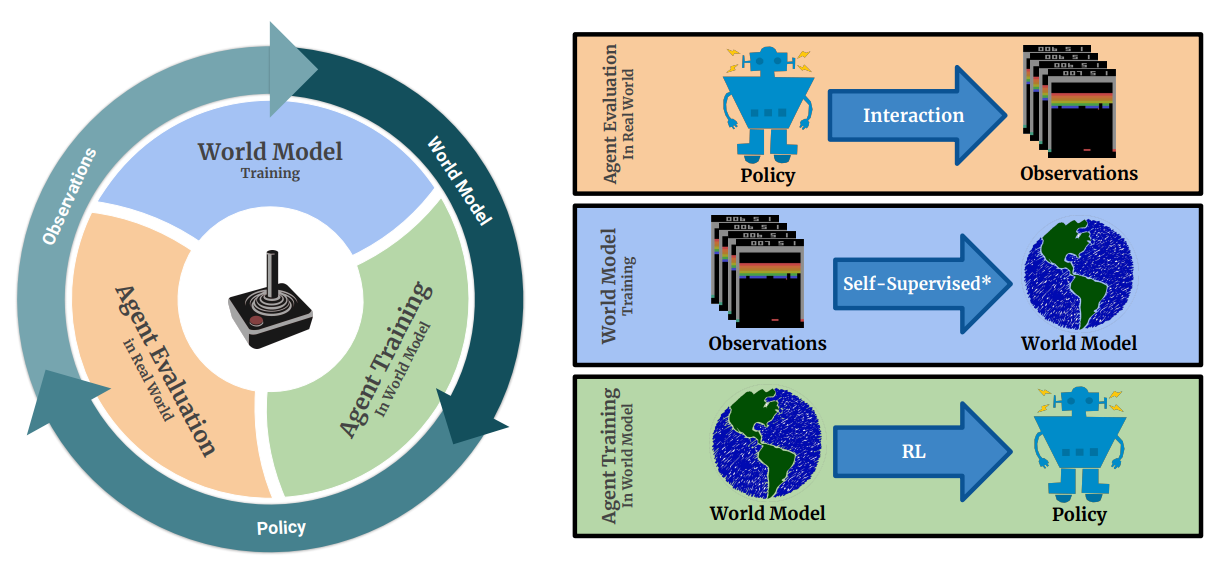
\includegraphics[width=0.8\columnwidth]{./figures/chapter_2/SimPLe.png}
        \caption{Simulación de entorno para la aceleración del aprendizaje.}\label{fig:rl_simple}
    \end{figure}
    
    En cada iteración:\\
    \begin{enumerate}
        \item El agente comienza a interactuar con el entorno real siguiendo el última política (inicializada al azar).\\
        \item Las observaciones recogidas se utilizarán para entrenar (actualizar) el mundo actual modelo.\\
        \item El agente actualiza la política actuando dentro del modelo mundial. La nueva política será evaluada para medir el rendimiento del agente así como recoger más datos.\\
        \item Vuelve al primer estado.\\
    \end{enumerate}
    
      Destacar que el entrenamiento del modelo global es auto-supervisado para los estados observados y supervisado para la recompensa.\\
    
    \item \textbf{Entrenamientos a través de los sueños}: El grupo de investigación DeepMind de Google\footnote{\url{https://deepmind.com/}} presentó una manera alternativa de entrenar algoritmos de aprendizaje por refuerzo. La situación que planteaban era sustituir un entorno de aprendizaje por refuerzo real por uno generado, entrenando al controlador del agente dentro de ese entorno creado por él, adquiriendo el aprendizaje en el mundo interno y transferir la política al entorno real. En el propio artículo de \textit{World Models}~\cite{world_models} permiten <<jugar>> con los parámetros para ver estos resultados\footnote{\url{https://worldmodels.github.io/}}. Puede verse una representación del mundo generado internamente en la figura \ref{fig:world_models}.\\
    
    \begin{figure}[!ht]
        \centering 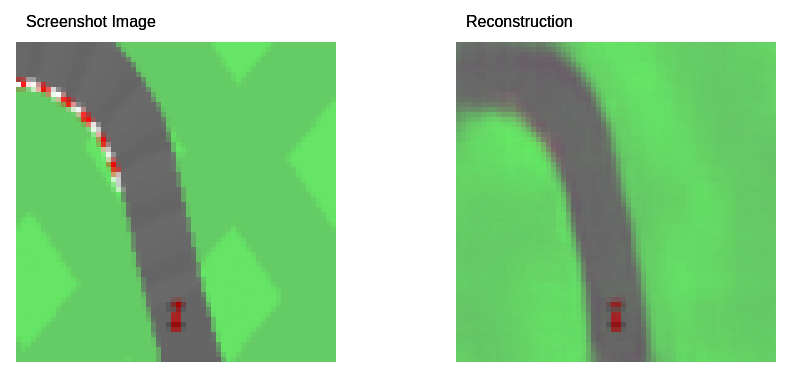
\includegraphics[width=0.6\columnwidth]{./figures/chapter_2/world_models.png}
        \caption{<<World Models>>. Generación de un entorno artificial para aprendizaje por refuerzo.}\label{fig:world_models}
    \end{figure}
    
    \item \textbf{Aprendizaje por refuerzo jerarquizado}: Igual que el aprendizaje profundo, se basa en las jerarquías de características. El aprendizaje por refuerzo jerarquizado (\textit{Hierarchical Reinforcement Learning}, \textit{HRL}) se basa en jerarquías de políticas donde, además de las acciones primitivas, también pueden aplicarse otras políticas (acciones en varias etapas). Este enfoque permite que las políticas de alto nivel se centren en objetivos de más alto nivel, mientras que las subpolíticas son responsables de un control preciso. El descubrimiento y la generalización de los objetivos es también un área importante de investigación en curso.\\
    
    En el trabajo de~\cite{hrl} se ven diferentes entornos donde un agente tiene que resolver un problema principal mientras resuelve problemas secundarios pero necesarios para finalizar el ejercicio. Puede verse un fragmento de una ilustración del trabajo en la figura \ref{fig:hrl}.\\

    \begin{figure}[!ht]
        \centering 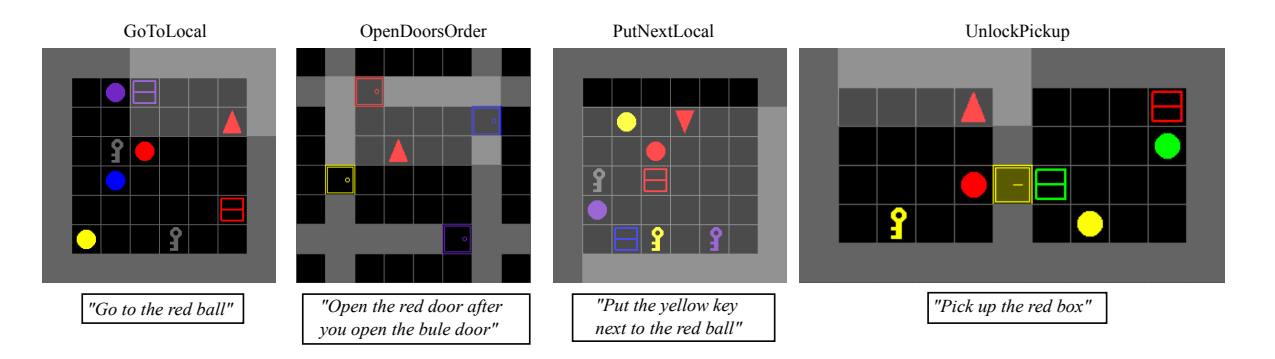
\includegraphics[width=0.9\columnwidth]{./figures/chapter_2/hrl.png}
        \caption{Aprendizaje por refuerzo jerarquizado. Resuelve pequeñas sub-tareas para resolver una mayor.}\label{fig:hrl}
    \end{figure}

    \item \textbf{Imitación y aprendizaje por refuerzo inverso}: El objetivo del aprendizaje por refuerzo inverso \textit{Inverse Reinforcement Learning}, IRL en adelante) e imitación (\textit{Imitation Learning}) es estimar una función de recompensa desconocida de las trayectorias observadas que caracterizan una solución~\cite{mohamed_medhat}. IRL puede ser usado en combinación con aprendizaje por refuerzo para mejorar en un comportamiento demostrado. Con el uso de las redes neuronales es posible aprender recompensas complejas y no lineales. Se demostró que las políticas se caracterizan de manera única por sus ocupaciones (estados visitados y distribución de acciones), lo que permite reducir el IRL al problema de la correspondencia de las medidas. Con esto y el uso de redes adversarias generativas se facilita recompensar el aprendizaje funcional de una manera más flexible, lo que resulta en el algoritmo de aprendizaje por imitación generativa adversaria (\textit{Generative Adversarial Imitation Learning}, GAIL). Este tipo de técnicas son muy empleadas para el entrenamiento de redes para el aprendizaje de coches autónomos, donde dado un comportamiento el coche <<hereda>> la información como en el trabajo de~\cite{oliver_cameron} con los coches autónomos.\\
    
    \item \textbf{Multi-agente}: El aprendizaje por refuerzo multiagente (\textit{Multi-Agent Reinforcement Learning}, MARL en adelante) considera el aprendizaje de múltiples agentes~\cite{nando_de_freitas} y la no estacionariedad introducida por otros agentes cambia su comportamiento a medida que aprenden. En DRL, el enfoque se ha centrado en permitir la comunicación (diferenciable) entre los agentes, lo que les permite cooperar. Un trabajo muy popular del multiagente es la solución que presentó OpenAI-Gym al juego del pilla-pilla (o \textit{hide and seek})~\cite{world_models}. En esta solución, un grupo de agentes adquiere el rol de <<buscadores>> para tratar de encontrar a otro grupo de agentes que se ocultarán en el entorno permitiéndose incluso el movimiento de objetos dentro del escenario como ayuda de camuflaje (paredes, cajas, etc). Una vez pasado el periodo de entrenamiento los agentes encargados de buscar consiguen encontrar a sus rivales que a su vez adquieren mejores habilidades para esconderse. Puede verse un conjunto de situaciones en la figura \ref{fig:multiagente-1}.
    
    \begin{figure}[!ht]
        \centering 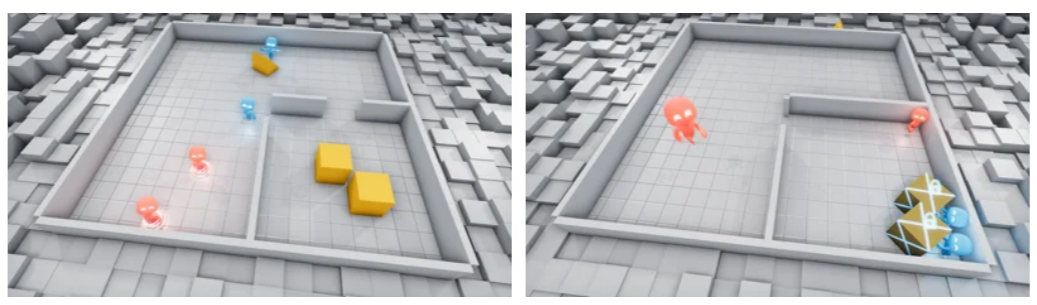
\includegraphics[width=0.8\columnwidth]{./figures/chapter_2/multiagente-1.png}
        \caption{Juego de \textit{hide and seek} utilizando aprendizaje por refuerzo profundo (OpenAI-Gym).}\label{fig:multiagente-1}
    \end{figure}
    
    Lo sorprendente de este trabajo es que cuando aumentan considerablemente los episodios de entrenamiento (las partidas) ambos grupos llevan al extremo el entorno de simulación llegando incluso a sobrepasar los límites de las físicas desarrolladas originalmente y todo con el objetivo de buscar o esconderse mejor. En la figura \ref{fig:multiagente-2} puede verse al agente encargado de buscar cómo utiliza uno de los objetos para elevarse y encontrar mejor a los agentes escondidos.\\
    
    \begin{figure}[!ht]
        \centering 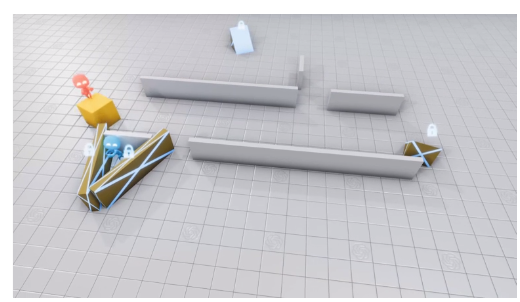
\includegraphics[width=0.5\columnwidth]{./figures/chapter_2/multiagente-2.png}
        \caption{Juego de \textit{hide and seek} utilizando aprendizaje por refuerzo profundo (OpenAI-Gym).}\label{fig:multiagente-2}
    \end{figure}

    \item \textbf{Transferencia de conocimiento (\textit{transfer learning}}): Aunque los algoritmos DRL pueden procesar entradas de alta dimensión, raramente es factible entrenar a los agentes de RL directamente en entradas visuales en el mundo real, debido al gran número de muestras requeridas. Para acelerar el aprendizaje en DRL, es posible explotar los conocimientos adquiridos previamente a partir de tareas relacionadas, que se presentan en varias formas: transferencia aprendizaje, aprendizaje multitarea~\cite{eric_tzeng} y aprendizaje curricular~\cite{ronan_collobert}, entre otros. Es muy interesante transferir el aprendizaje de una tarea a otra, particularmente del entrenamiento en simuladores de física con renderizadores visuales para el posterior ajuste de los modelos en el mundo real. Esto puede lograrse utilizando directamente la misma red tanto en la fase de simulación como en la fase real con procedimientos de formación más sofisticados que intentan mitigar directamente el problema de las redes neuronales ``olvidando'' el viejo conocimiento añadiendo capas adicionales al transferir el dominio (cabezal).\\
    
    En la figura \ref{fig:transfer-learning} puede verse un diagrama donde de izquierda a derecha se entrena la misma red con pesos vacíos (sin conocimiento previo), una red central con un entrenamiento para resolver el problema de <<Image-Net>> y ajustando en un nuevo entrenamiento la última red al problema que se quiere resolver. Por ejemplo, clasificar imágenes no vistas por el conjunto de datos original pero con todo el conocimiento adquirido del entrenamiento previo. 
     
    \begin{figure}[!ht]
        \centering 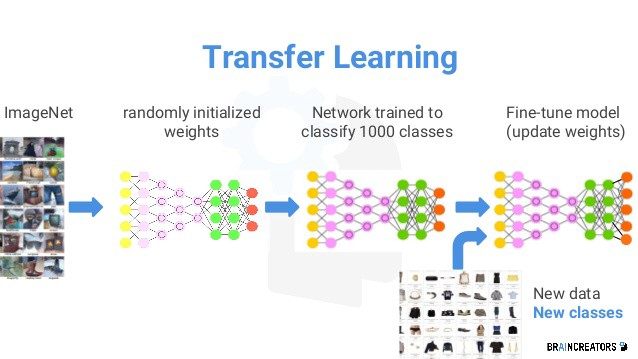
\includegraphics[width=0.7\columnwidth]{./figures/chapter_2/transfer-learning.jpeg}
        \caption{Transferencia de aprendizaje.}\label{fig:transfer-learning}
    \end{figure}
\end{itemize}




